\documentclass[aspectratio=169]{beamer}
\usetheme{default}
\setbeamertemplate{navigation symbols}{}
\usepackage{tikz}
\usepackage{eurosym}

\title{Research with AI Agents}
\subtitle{What Works, What It Costs, and What an Institute Needs}
\author{Lukas Theissinger}
\date{\today}

\AtBeginSection[]{
  \begin{frame}{Outline}
    \tableofcontents[currentsection]
  \end{frame}
}

\usetikzlibrary{calc}
\begin{document}

\begin{frame}
  \titlepage
\end{frame}

\begin{frame}{Outline}
  \tableofcontents
\end{frame}

% 1. ~6 min
\section{OpenAI and Agent Usage}

\begin{frame}{FOMO Headline: OpenAI Agent Usage}
  \centering
  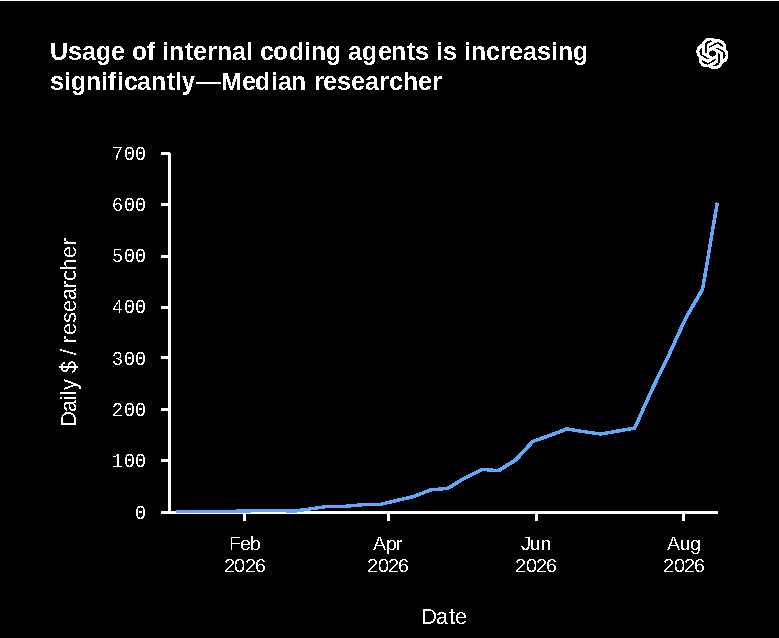
\includegraphics[height=0.78\textheight]{assets/openai-median-usage.pdf}\\[2pt]
  {\tiny Median researcher, daily \$ spent on internal coding agents.
  Source: OpenAI, ``Research acceleration'' (self-reported).}
\end{frame}

\begin{frame}{What do agents do at OpenAI?}
% --- Reading of the chart (speaker notes, not shown) -----------------------
% What it shows: increase in OUTPUT TOKENS per researcher per day since
% the start of 2026, split into 18 research activities (6 groups).
% Values from the chart's data labels; total ~ +654k tokens/day.
% Top 3 bars = 75% of the increase:
%   3.1 Research & infrastructure code   +198k (30%)
%   6.2 Technical help & review          +159k (24%)
%   4.1 Launch, monitor & debug runs     +133k (20%)
% Next: 5.1 Analyze experiment results +40k, 4.2 Compute-cluster ops +37k;
%   everything else below +20k.
% By group (sum of bars):
%   Build ~212k (32%) | Communicate ~185k (28%, almost all 6.2) |
%   Run ~183k (28%)   | Analyze ~55k (8%) | Design ~15k (2%) | Decide ~4k (<1%)
% Takeaway for the talk:
%   1. Agents took over the DOING -- writing code, running/debugging jobs,
%      answering technical questions. Fits the chart: these tasks are
%      token-heavy by nature, so the big bars are expected.
%   2. Did agents take over the THINKING? The chart can't tell us. What to
%      work on +2.3k, continue or stop +0.2k, planning +5.1k, reviewing
%      external research +0.7k -- but even fully AI-driven, these tasks
%      produce short outputs (a decision, a plan, a summary). Output tokens
%      are the wrong measure here; small bars != little use.
%   3. What we CAN say: every one of the 18 activities went up -- agents are
%      used everywhere in the research process. HOW MUCH and HOW EXACTLY
%      they are used for the thinking parts stays open.
% Caveats: self-reported by OpenAI; tokens measure volume, not value;
%   absolute increase, so small categories may still have grown a lot
%   in %; how calls were assigned to categories is not stated.
% --------------------------------------------------------------------------
  \centering
  \begin{tikzpicture}
    \node[anchor=south west, inner sep=0] (chart)
      {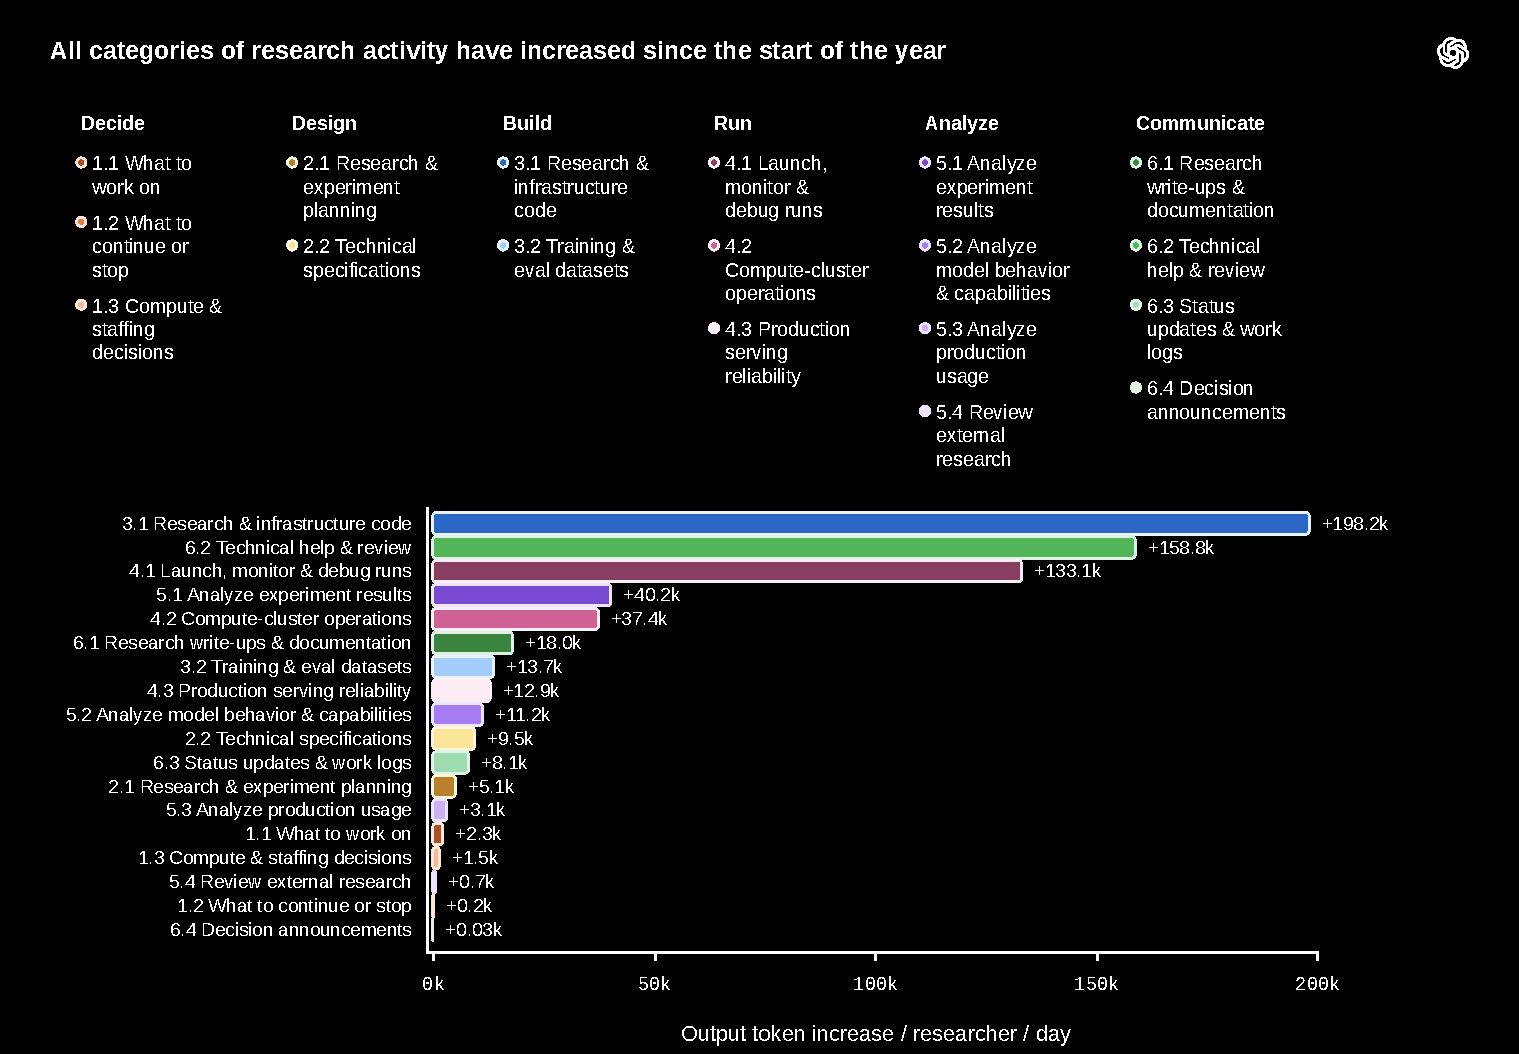
\includegraphics[height=0.78\textheight]{assets/openai-usage-categories.pdf}};
    % click 2: vector zoom on the bar chart and its x axis, rest stays visible
    \only<2>{
      \node[inner sep=0, fill=black] (zoom) at ([yshift=-4pt]chart.center)
        {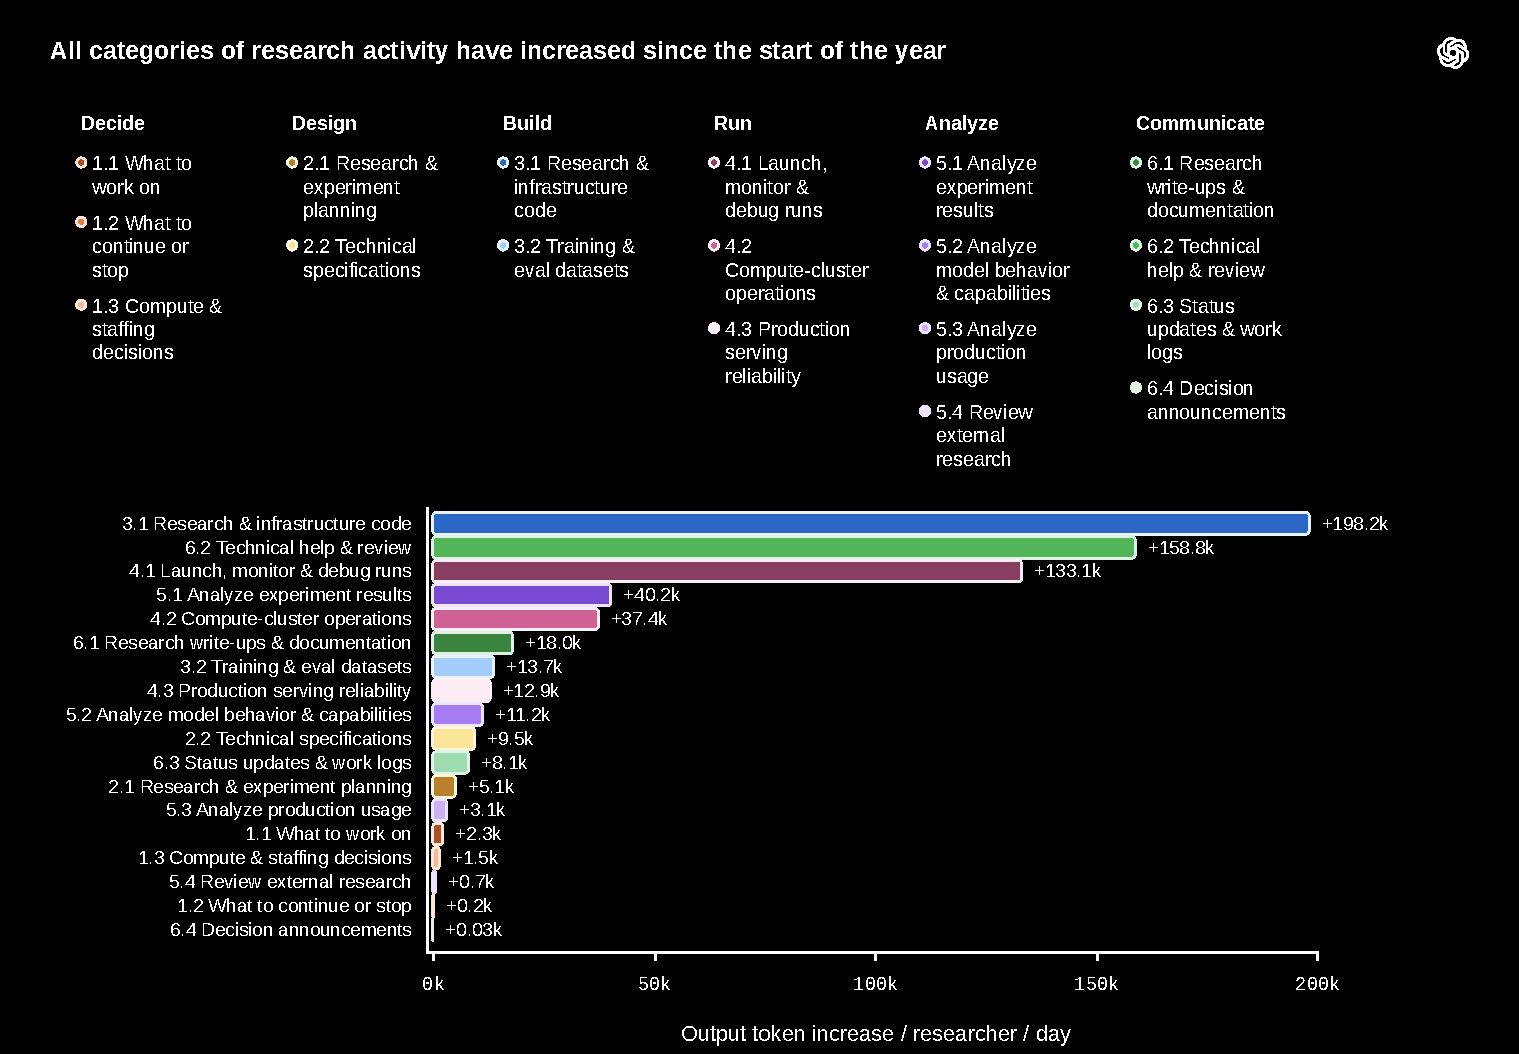
\includegraphics[width=0.98\textwidth, trim=22 2 58 238, clip]{assets/openai-usage-categories.pdf}};
      % cut between 6.3 Status updates (doing) and 2.1 Research planning (thinking)
      \coordinate (cl) at ($(zoom.south west)!0.491!(zoom.north west)$);
      \coordinate (cr) at ($(zoom.south east)!0.491!(zoom.north east)$);
      \draw[red, line width=1.5pt, dashed] (cl) -- (cr);
      \node[red, font=\bfseries\small, anchor=south east] at ($(cl)!0.98!(cr)$) {doing $\uparrow$};
      \node[red, font=\bfseries\small, anchor=north east] at ($(cl)!0.98!(cr)$) {thinking $\downarrow$};
    }
  \end{tikzpicture}\\[2pt]
  {\tiny Increase in output tokens per researcher per day, by research activity.
  Source: OpenAI, ``Research acceleration'' (self-reported).}
\end{frame}

% Speaker notes (Tim Dettmers, "Use Agents or Be Left Behind? A Personal Guide
% to Automating Your Own Work", 2026-01-13; quotes checked against the post):
%   - Claim, after 8 months of Claude Code: "more than 90% of code and text
%     should be written by agents. You need to do so, or you will be left behind."
%   - His blog posts are >95% AI-generated. A post now takes ~3 h: 1 h speaking
%     into a microphone, 10 min agent workflow, ~2 h reviewing and editing.
%   - Degree of automation: "You always have a degree of automation." Raise it
%     only where it pays: how often you do the task x time saved vs. the time
%     to automate it (process optimization: stopwatch on the factory floor).
%     "There are many tasks that should not be automated because it is not
%     effective."
%   - Failure: two months on an email agent; "I could not get any degree of
%     automation improvement by using agents for emails."
%   - Decisions stay human: "there will always be work where your personal
%     preferences, decisions, and taste will be needed -- even if 90% of the
%     work happens through AI."
%   - Conclusion: "agent use is a skill, and like any skill, it requires
%     deliberate practice, understanding of when it applies, and acceptance
%     that you will fail often before you succeed."

\begin{frame}{Dettmers' Interpretation}
  {\small Tim Dettmers' hypotheses, read against the OpenAI usage data}
  \vspace{6pt}
  \renewcommand{\arraystretch}{1.35}
  \footnotesize
  % Clicks 1-4: what the chart suggests (left), one row per click.
  % Clicks 5-8: what Dettmers says (right), one row per click.
  % (\leavevmode keeps the \uncover cells top-aligned with the plain ones)
  \begin{tabular}{@{}p{0.49\textwidth}p{0.45\textwidth}@{}}
    \textbf{What the OpenAI chart suggests}
      & \leavevmode\uncover<5->{\textbf{Dettmers says}} \\ \hline
    All 18 activities went up: agents are used everywhere,
        but how much and how exactly is still open.
      & \leavevmode\uncover<5->{Use agents or be left behind.} \\
    \leavevmode\uncover<2->{Agents took over the \emph{doing}: code, runs, technical help.}
      & \leavevmode\uncover<6->{``More than 90\% of code and text should be written by agents.''} \\
    \leavevmode\uncover<3->{Frequent, repetitive work grew most; rare decisions grew least.}
      & \leavevmode\uncover<7->{Automate only if how often $\times$ time saved $>$ time to build.} \\
    \leavevmode\uncover<4->{Did agents take over the \emph{thinking}? We can't say:
        a plan or a decision is short, so tokens are the wrong measure.}
      & \leavevmode\uncover<8->{Agent use is a \emph{skill}: not everything can or should
        be automated (degree of automation).} \\
  \end{tabular}
  \vfill
  {\tiny Sources: timdettmers.com/2026/01/13/use-agents-or-be-left-behind;
  OpenAI, ``Research acceleration'' (self-reported).}
\end{frame}

% Field report (speaker notes). Sources: github.com/Newida/AutomatingExercises
% (README, commit history) and the first real run on an exercise sheet (2026-10-26).
%   - Why this task: every exercise sheet repeats the same work (read, solve, code,
%     plot, make slides), so by Dettmers' rule it is worth automating. The README
%     says the approach follows his guide.
%   - How: one command; the PDF is the only input (data files it names are looked
%     up next to it). Three agent runs (Claude Code by default, OpenAI Codex with
%     --agent codex): check inputs, solve, make slides. Agents never install
%     packages; the solver has no web access (Claude Code).
%   - First real run (solve stage only, Claude Code): 15 tasks, none partial or
%     blocked, $3.37 at API prices. Where the sheet prints reference values, the
%     results match them; the rest was not checked independently.
%   - It also flagged problems in the sheet itself: two typos, a loss that can go
%     negative, and weights that are not the maximum-likelihood ones.
%   - The slides were the hard part (15 of 25 commits): first one deck by hand,
%     then its structure written down sentence by sentence
%     (templates/slides/pattern.md) plus a personal style file (styles/lukas.md);
%     the hand-made deck was removed afterwards.
%   - Checking stays human: the solver grades its own work (confidence per task
%     in REPORT.md); read REPORT.md and slides/NOTES.md before class.
%   - Dettmers' rule for this tool: sheets per semester x time saved per sheet
%     vs. time to build (25 commits, Oct 26-29).

\begin{frame}{Field Report: Automating Exercises}
  % One step per click: problem, what is automated, what is left, link.
  \begin{enumerate}
    \setlength{\itemsep}{1em}
    \item<1-> \textbf{The problem.} PhD student, tutoring an exercise class every two weeks:
      \begin{itemize}\footnotesize
        \item 2\,h exercise class + 6\,h preparation (solving the tasks, making the slides)
        \item rough estimate: \textbf{2\,h + 6\,h = 8\,h every two weeks}
      \end{itemize}
    \item<2-> \textbf{Automate as much as possible.}
      \begin{itemize}\footnotesize
        \item[a)] Task solving: an agent solves every task, with code and plots
        \item[b)] Slide creation: an agent turns the solutions into the class slides
      \end{itemize}
    \item<3-> \textbf{Left to do:} understand the solutions, make small updates to the slides.
      \begin{itemize}\footnotesize
        \item class stays 2\,h, preparation drops from 6\,h to 2\,h: \textbf{2\,h + 2\,h = 4\,h every two weeks}
      \end{itemize}
    \item<4-> \textbf{Ask your agent to try it:}
      \href{https://github.com/Newida/AutomatingExercises}{\texttt{github.com/Newida/AutomatingExercises}}\
      {\color{red}\textbf{Avoid:} Don't do anything BY HAND on this project. If you want to change it, ASK YOUR AGENT to change it.}
  \end{enumerate}
\end{frame}

% 2. ~6 min
\section{Owning Intelligence and Infrastructure at Lamarr}

\begin{frame}{Automating at Bigger Scale}
  \begin{itemize}
    \item<1-> \textbf{So far:} each of us automates our own tasks.
    \item<2-> \textbf{Share it:} one person builds it, everyone reuses and adapts it to their needs.
    \item<3-> \textbf{Institute level:} tasks that never pay off for one person start to pay off.
  \end{itemize}
  \medskip
  \uncover<4->{%
  \begin{block}{Example: travel expense reports}
    \small Collect receipts, fill in the university form, look up per-diem rules, fix what admin sends back: say \textbf{3 trips $\times$ 3\,h per person per year}. An agent that reads the receipts and files the form correctly needs \textbf{$\sim$200\,h} (rules, forms, access to the admin system).\par\smallskip
    \centering
    \begin{tabular}{lccc}
      & how often $\times$ time saved & time to build & \\ \hline
      \uncover<5->{one person} & \uncover<5->{$3 \times 3$\,h $= 9$\,h/year} & \uncover<5->{200\,h} & \uncover<5->{\textcolor{red}{\textbf{never pays}}} \\
      \uncover<6->{institute, 10\,000 people} & \uncover<6->{$10\,000 \times 9$\,h $= 90\,000$\,h/year} & \uncover<6->{200\,h} & \uncover<6->{\textcolor{green!50!black}{\textbf{pays $>$400$\times$}}} \\
    \end{tabular}
  \end{block}}
\end{frame}
% Notes: Dettmers' rule (how often x time saved > time to build) applied once
% per person vs. once for the whole institute. Numbers are rough illustrations.
% Also: only the institute can build it -- it needs the official form and admin-system access.

\begin{frame}{What Agents Cost}
  \begin{itemize}
    \item<1-> \textbf{Me:} Claude \emph{and} Codex, 20\,\euro{} plan each: \textbf{40\,\euro{} per month}.
      One plan alone is not enough.
    \item<2-> \textbf{Colleagues:} 100\,\euro{} Claude plan, and they hit its limit \textbf{every week}.
    \item<3-> \textbf{As we have seen:} every Lamarr member needs AI agents.
      You cannot work without them anymore.
  \end{itemize}
  \medskip
  \uncover<4->{{\small\color{red}
    \textbf{Dear management:} do not assume that employees will continue spending their own money.
    We are bottlenecking ourselves: we don't want to spend 100\,\euro{} per month just to do our work,
    so we spend 20\,\euro{}, effectively leaving performance on the table.
    Also, people will just switch to other institutes, even outside Germany,
    that supply them with the AI they want and need, for free, to get important work done.\par}}
  \medskip
  \uncover<5->{\centering\Large So let's talk about costs.\par}
\end{frame}
% Notes: "If you still cannot see it, you are super delusional."
% Two decisions follow: 1) subscription vs. API (individual), 2) self-hosting (institute only).

\begin{frame}{Decision 1: Subscription or API?}
  \small
  \begin{columns}[T]
    \begin{column}{0.48\textwidth}
      \uncover<1->{\textbf{Subscription} (20--200\,\euro{}/month)
      \begin{itemize}
        \item[+] flat price, no surprise bills
        \item[+] very cheap for heavy interactive use
        \item[--] usage caps (5-hour and weekly)
        \item[--] one person, one login; not for pipelines
      \end{itemize}}
    \end{column}
    \begin{column}{0.48\textwidth}
      \uncover<2->{\textbf{API} (pay per token)
      \begin{itemize}
        \item[+] no caps, run many agents in parallel
        \item[+] scripts, batch jobs, shared tools
        \item[--] heavy daily use gets expensive fast
        \item[--] needs a budget and someone watching it
      \end{itemize}}
    \end{column}
  \end{columns}
  \medskip
  % TODO: cost comparison. The ~680$ (Claude) and ~145$ (Codex) are rough estimates from my
  %   usage logs at list prices (token prices not verified), not invoices. Replace with a
  %   measured subscription-vs-API comparison: same tasks run both ways (planned QHack run,
  %   branch ai/qhack-sub-vs-api-20261021, commit 0343df1, not run yet); check current prices.
  \uncover<3->{%
  \begin{block}{Our comparison: one month of my usage, priced at API list prices}
    \centering
    \begin{tabular}{lccc}
      & subscription & same usage via API & factor \\ \hline
      Claude & 20\,\$ (Pro) & $\sim$680\,\$ & $\sim$34$\times$ \\
      Codex  & 20\,\$ (Plus) & $\sim$145\,\$ & $\sim$7$\times$ \\
    \end{tabular}\par\smallskip
    \raggedright But one batch job, 27 benchmark tasks via API, cost only \textbf{2.25\,\$}.
  \end{block}}
  \uncover<4->{\textbf{Rule of thumb:} people $\to$ subscription; pipelines and batch jobs $\to$ API.}
\end{frame}
% Notes: API figures are estimates from my own usage log at list prices, not invoices.
% The 2.25 $ is the QHack 27-task run with gpt-6.1-sol via API.

\begin{frame}{Decision 2: Self-Hosting Open Models}
  \small
  \begin{itemize}
    \item<1-> \textbf{Not for individuals}, but realistic for Lamarr: the institute already runs large GPU clusters.
    \item<2-> \textbf{Open-weight models:} Qwen (Alibaba), DeepSeek, GPT-OSS (OpenAI), Kimi (Moonshot), GLM (Zhipu), Mistral.
    \item<3-> \textbf{Go big, not small:} the frontier-class open models (0.5--1T parameters, e.g.\ DeepSeek, Kimi, GLM, Qwen-Coder)
      need $\sim$1\,TB of GPU memory per copy: one or two full 8-GPU nodes, several of them to serve everyone.
  \end{itemize}
  \medskip
  \uncover<4->{%
  \begin{block}{Quality: our quantum-coding benchmark (27 tasks, solved), so far only small open models}
    \centering
    \begin{tabular}{lc}
      Qwen, self-hosted on one GPU & 10/27 \\
      GPT-OSS, self-hosted on one GPU & 12--15/27 \\
      GPT-5-nano (small cloud model) & 14/27 \\
      frontier cloud model (GPT-6.1-sol) & \textbf{26/27} \\
    \end{tabular}
  \end{block}}
  \uncover<5->{Small open models are clearly behind. The largest open models are much closer to the frontier;
  on our tasks they are \textbf{still untested}.}
\end{frame}
% Notes: GPT-OSS 12/27 with 2K context, 15/27 with 8K context. One benchmark, our own tasks;
% indicates the gap, not a general ranking. Only single-GPU models were tested; a 0.5-1T open model
% on the cluster has not been run on these tasks. "Much closer to the frontier" = public leaderboards
% (gap of months, not years), not our own measurement.

\begin{frame}{Self-Hosting for the Institute: Pros and Cons}
  \footnotesize
  \begin{columns}[T]
    \begin{column}{0.48\textwidth}
      \textbf{Quality and performance}
      \begin{itemize}
        \item<1->[+] data never leaves Lamarr (privacy, unpublished work, GDPR)
        \item<1->[+] no vendor caps or outages, models don't change under you
        \item<1->[+] fine-tune on our own data, research on the models themselves
        \item<2->[--] even the best open models trail the closed frontier (by months), most on hard agentic tasks
        \item<2->[--] slower when many people use it at once
      \end{itemize}
    \end{column}
    \begin{column}{0.48\textwidth}
      \textbf{Costs}
      \begin{itemize}
        \item<3->[+] no per-token bill: more use costs nothing extra
        \item<3->[+] shared by all members, predictable budget
        \item<3->[+] Lamarr already has the GPUs and the people who run them
        \item<4->[--] a frontier-class model occupies whole nodes around the clock, taken from research jobs
        \item<4->[--] power, cooling and staff to run it
        \item<4->[--] hardware ages in 3--5 years; idle at night
      \end{itemize}
    \end{column}
  \end{columns}
  \medskip
  \uncover<5->{%
  \begin{block}{Rough comparison}
    \centering 2 nodes $\times$ 300\,k\euro{} over 4 years $\approx$ 12.5\,k\euro{}/month
    $\approx$ \textbf{300 people $\times$ 40\,\euro{}} $\approx$ \textbf{125 people $\times$ 100\,\euro{}}
    \par\smallskip\raggedright With Lamarr's compute, a frontier-class open model for everyone is realistic:
    it pays off through privacy, scale and no caps; the closed models keep a lead of months.
  \end{block}}
\end{frame}
% Notes: 300 k EUR is an illustrative 8-GPU-node price, not a quote; excludes power and staff.
% 2 nodes = roughly one copy of a ~1T-parameter model; serving hundreds of users needs more.

% Takeaways (one per click), grouped by the three questions in the subtitle.
% Where each one comes from:
%   - doing vs. decisions: OpenAI chart + Dettmers ("decisions, and taste will be
%     needed -- even if 90% of the work happens through AI"); checking: Field Report.
%   - 6 h -> 2 h: my own estimate (Field Report), every two weeks.
%   - costs: What Agents Cost, Decision 1 (API figures are rough, see TODO there).
%   - 10 000 people: travel-expense example, illustrative numbers.
%   - open model: Decision 2 + Pros/Cons; realistic with Lamarr's GPUs, months
%     behind the closed frontier, not yet tested on our tasks.
\begin{frame}{Takeaways}
  \begin{columns}[T]
    \begin{column}{0.54\textwidth}
      \uncover<1->{\structure{\textbf{For the individual}}}
      \begin{enumerate}
        \setlength{\itemsep}{0.6em}
        \item<1-> \textbf{You need to use AI agents.}
        \item<2-> \textbf{Use AI agents as much as possible.}
        \item<3-> \textbf{Automate, to a degree, only what pays off:}\\[2pt]
          {\small$\text{how often} \times \text{time saved} > \text{time to build}$}
        \item<4-> \textbf{Agent use is a skill} you need to learn.
      \end{enumerate}
    \end{column}
    \begin{column}{0.44\textwidth}
      \uncover<5->{\structure{\textbf{For the institute}}}
      \begin{enumerate}
        \setlength{\itemsep}{0.6em}
        \item<5-> \textbf{Automate workflows for every individual:} what never pays off for one person pays off for 10\,000.
        \item<6-> \textbf{Provide your employees with agents.}
        \item<7-> \textbf{Consider self-hosting.}
      \end{enumerate}
    \end{column}
  \end{columns}
\end{frame}

% 3. ~3 min -- optional: kept last so it can be cut if time runs short
\section{Staying Up to Date with AI}

\begin{frame}{How to Stay Up to Date}
  \begin{enumerate}
    \setlength{\itemsep}{1.2em}
    \item \textbf{Make an X (Twitter) account.}\\
      Many people from the frontier labs post there first, often daily.
    \item \textbf{Read ``Today's News'' on the home page.}\\
      It sums up the biggest updates of the day.
    \item \textbf{Follow the right people.}\\
      Don't be fooled by clickbait.
  \end{enumerate}
\end{frame}

\begin{frame}{Read Today's News}
  \centering
  \begin{tikzpicture}
    \node[anchor=south west, inner sep=0] (shot)
      {
\includegraphics[height=0.78\textheight]{assets/x-news-and-reset.png}};
    \begin{scope}[x={(shot.south east)}, y={(shot.north west)}]
      % boxes as fractions of the screenshot size
      \draw[red, line width=2pt, rounded corners=3pt] % Tibo's reset post
        (0.232, 0.676) rectangle (0.686, 0.768);
      \draw[red, line width=2pt, rounded corners=3pt] % Today's News
        (0.718, 0.020) rectangle (0.995, 0.496);
      % click 2: zoom on Today's News, click 3: zoom on Tibo's reset
      \fill<2->[white, opacity=0.7] (0,0) rectangle (1,1);
      \node<2>[inner sep=0] at (0.5, 0.5)
        {
\includegraphics[height=0.74\textheight]{assets/zoom-todays-news.png}};
      \node<3>[inner sep=0] at (0.5, 0.5)
        {
\includegraphics[width=0.9\textwidth]{assets/zoom-tibo-reset.png}};
    \end{scope}
  \end{tikzpicture}
\end{frame}

\begin{frame}{Who to Follow and Why}
  \small
  \renewcommand{\arraystretch}{1.35}
  \begin{tabular}{@{}l l p{0.5\textwidth}@{}}
    \textbf{Who} & \textbf{Handle} & \textbf{Why} \\ \hline
    Andrej Karpathy   & @karpathy     & Clear explanations of LLMs and how to work with them \\
    Thibault Sottiaux (tibo) & @thsottiaux & Leads OpenAI Codex; news on Codex releases and usage limits \\
    Boris Cherny      & @bcherny      & Created Claude Code; how Anthropic uses its own agents \\
    Tim Dettmers      & @Tim\_Dettmers & Agents in academic research; open models on small budgets \\
    Victor Taelin     & @VictorTaelin & Tests frontier models on hard coding problems \\
    Felix Rieseberg   & @felixrieseberg & Builds Claude's desktop apps at Anthropic; early product news \\
  \end{tabular}

  \vspace{1em}
  {\footnotesize\itshape A few of the 251 accounts I follow, all of this kind.}
\end{frame}

\begin{frame}{A Recent Headline You Might Have Missed}
  \centering
  \begin{tikzpicture}
    \node[anchor=south west, inner sep=0] (shot)
      {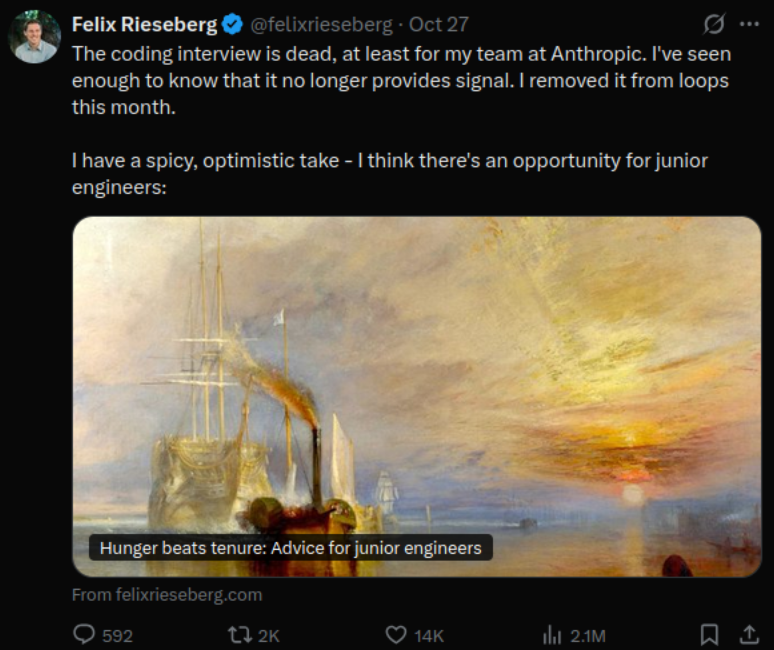
\includegraphics[height=0.82\textheight]{assets/felix-post-cropped.png}};
    \begin{scope}[x={(shot.south east)}, y={(shot.north west)}]
      % click 2: zoom on the first paragraph
      \fill<2>[white, opacity=0.7] (0,0) rectangle (1,1);
      \node<2>[inner sep=0] at (0.5, 0.6)
        {
\includegraphics[width=0.95\textwidth]{assets/zoom-felix-headline.png}};
    \end{scope}
  \end{tikzpicture}
\end{frame}

\end{document}
